\documentclass{article}

\usepackage{graphicx}
\usepackage{amsmath}
\usepackage{fancyhdr}
\usepackage{listings}
\usepackage{xcolor}
\usepackage{textcomp}
\usepackage{float}
\usepackage[sorting=none]{biblatex}
\usepackage[margin=1in]{geometry}
\usepackage[font={small,it}]{caption}
\usepackage{placeins}
\usepackage{xepersian}

%\DeclareMathOperator*{\btie}{\bowtie}
\addbibresource{bibliography.bib}
\settextfont[Scale=1.2]{B-NAZANIN.TTF}
\setlatintextfont[Scale=1]{Times New Roman}
\renewcommand{\baselinestretch}{1.5}
\pagestyle{fancy}
\fancyhf{}
\rhead{تکلیف ششم درس پایگاه داده‌ها 1}
\lhead{\thepage}
\rfoot{علیرضا ابره فروش}
\lfoot{9816603}
\renewcommand{\headrulewidth}{1pt}
\renewcommand{\footrulewidth}{1pt}
%%%%%%%%%%
\lstset
{
    language=[latex]tex,
    basicstyle=\ttfamily,
    commentstyle=\color{black},
    columns=fullflexible,
    keepspaces=true,
    upquote=true,
    showstringspaces=false,
    morestring=[s]\\\%,
    stringstyle=\color{black},
}
%%%%%%%%%%

\begin{document}
\begin{titlepage}
\begin{center}

\includegraphics[width=0.4\textwidth]{figures/IUT Logo.png}\\
        
\LARGE
\textbf{دانشگاه صنعتی اصفهان}\\
\textbf{دانشکده مهندسی برق و کامپیوتر}\\
        
\vfill
        
\huge
\textbf{عنوان: تکلیف چهارم درس ریزپردازنده}\\
        
\vfill
        
\LARGE
\textbf{نام و نام خانوادگی: علیرضا ابره فروش}\\
\textbf{شماره دانشجویی: 9816603}\\
\textbf{نیم\,سال تحصیلی: پاییز 1400}\\
\textbf{مدرّس: دکتر عارف کریمی افشار}\\
\end{center}
\end{titlepage}


%\tableofcontents
\newpage


\section{1}
\begin{figure}[H]
    \centering
    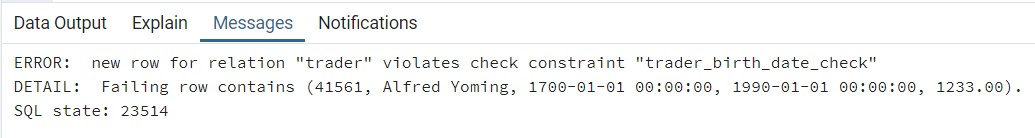
\includegraphics[width=1\textwidth]{figures/1.jpg}
    \caption
	{
سوال 1
	}
    \label{fig:fig1}
\end{figure}


\section{2}


\section{3}
\begin{figure}[H]
    \centering
    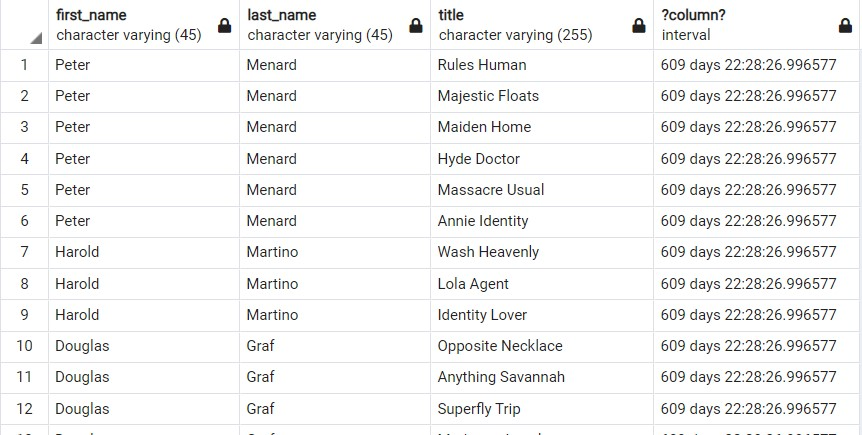
\includegraphics[width=1\textwidth]{figures/3.jpg}
    \caption
	{
سوال 3
	}
    \label{fig:fig1}
\end{figure}


\section{4}
سه روش اصلیِ \lr{Blob}، \lr{Clob} و ذخیره در دیسک و استفاده از پوینتر برای درسترسی به فایل است.
\begin{latin}
\begin{table}[H]
\centering
\caption{}
\label{tab:my-table}
\begin{tabular}{|c|l|l|}
\hline
\textbf{}   & \multicolumn{1}{c|}{\textbf{Blob}}                                                                                                        & \multicolumn{1}{c|}{\textbf{Clob}}                                                                                                           \\ \hline
\textbf{1.} & \begin{tabular}[c]{@{}l@{}}The full form of Blob is\\ a Binary Large Object.\end{tabular}                                                 & \begin{tabular}[c]{@{}l@{}}The full form of Clob is\\ Character Large Object.\end{tabular}                                                   \\ \hline
\textbf{2.} & \begin{tabular}[c]{@{}l@{}}This is used to store\\ large binary data.\end{tabular}                                                        & \begin{tabular}[c]{@{}l@{}}This is used to store\\ large textual data.\end{tabular}                                                          \\ \hline
\textbf{3.} & \begin{tabular}[c]{@{}l@{}}This stores values in the\\ form of binary streams.\end{tabular}                                               & \begin{tabular}[c]{@{}l@{}}This stores values in the form\\ of character streams.\end{tabular}                                               \\ \hline
\textbf{4.} & \begin{tabular}[c]{@{}l@{}}Using this you can stores\\ files like videos, images,\\ gifs, and audio files.\end{tabular}                   & \begin{tabular}[c]{@{}l@{}}Using this you can store files\\ like text files, PDF documents,\\ word documents etc.\end{tabular}               \\ \hline
\textbf{5.} & \begin{tabular}[c]{@{}l@{}}MySQL supports this with\\ the following datatypes:\\ TINYBLOB\\ BLOB\\ MEDIUMBLOB\\ LONGBLOB\end{tabular}     & \begin{tabular}[c]{@{}l@{}}MySQL supports this with the\\ following datatypes:\\ TINYTEXT\\ TEXT\\ MEDIUMTEXT\\ LONGTEXT\end{tabular}        \\ \hline
\textbf{6.} & \begin{tabular}[c]{@{}l@{}}In JDBC API it is represented\\ by java.sql.Blob Interface.\end{tabular}                                       & \begin{tabular}[c]{@{}l@{}}In JDBC it is represented\\ by java.sql.Clob Interface.\end{tabular}                                              \\ \hline
\textbf{7.} & \begin{tabular}[c]{@{}l@{}}The Blob object in JDBC\\ points to the location of\\ BLOB instead of holding\\ its binary data.\end{tabular}  & \begin{tabular}[c]{@{}l@{}}The Blob object in JDBC\\ points to the location of\\ BLOB instead of holding\\ its character data.\end{tabular}  \\ \hline
\textbf{8.} & \begin{tabular}[c]{@{}l@{}}To store Blob JDBC\\ (PreparedStatement)\\ provides methods like:\\ setBlob()\\ setBinaryStream()\end{tabular} & \begin{tabular}[c]{@{}l@{}}To store Clob JDBC\\ (PreparedStatement)\\ provides methods like:\\ setClob()\\ setCharacterStream()\end{tabular} \\ \hline
\textbf{9.} & \begin{tabular}[c]{@{}l@{}}And to retrieve\\ (ResultSet) Blob\\ it provides methods\\ like:\\ getBlob()\\ getBinaryStream\end{tabular}    & \begin{tabular}[c]{@{}l@{}}And to retrieve\\ (ResultSet) Clob it\\ provides methods\\ like:\\ getClob()\\ getCharacterStream()\end{tabular}  \\ \hline
\end{tabular}
\end{table}
\end{latin}

\section{5}
\begin{figure}[H]
    \centering
    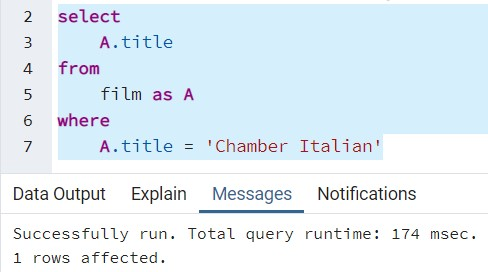
\includegraphics[width=1\textwidth]{figures/5-a.jpg}
    \caption
	{
کوئری پیش از تعریف ایندکس در 174 میلی‌ثانیه اجرا می‌شود.
	}
    \label{fig:fig1}
\end{figure}
\begin{figure}[H]
    \centering
    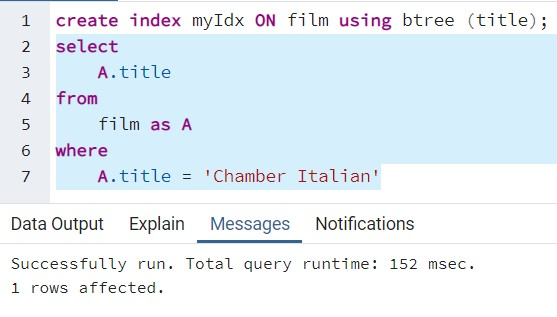
\includegraphics[width=1\textwidth]{figures/5-b.jpg}
    \caption
	{
کوئری پس از تعریف ایندکس در 152 میلی‌ثانیه اجرا می‌شود.
	}
    \label{fig:fig1}
\end{figure}
\begin{figure}[H]
    \centering
    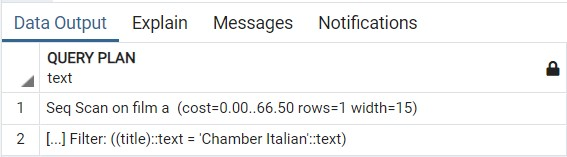
\includegraphics[width=1\textwidth]{figures/5-c.jpg}
    \caption
	{
خروجی \lr{explain} پیش از تعریف ایندکس
	}
    \label{fig:fig1}
\end{figure}
\begin{figure}[H]
    \centering
    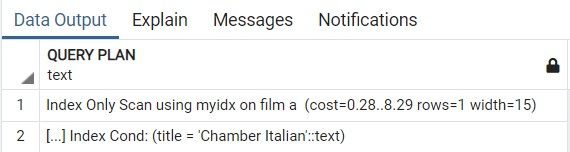
\includegraphics[width=1\textwidth]{figures/5-d.jpg}
    \caption
	{
خروجی \lr{explain} پس از تعریف ایندکس
	}
    \label{fig:fig1}
\end{figure}


\section{6}
\begin{figure}[H]
    \centering
    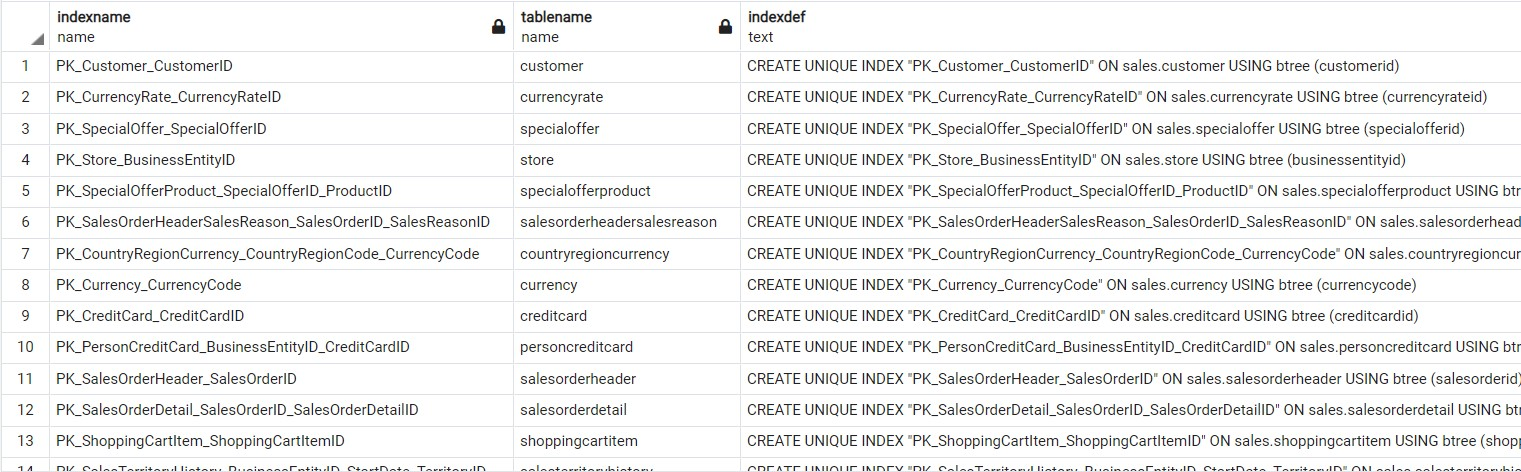
\includegraphics[width=1\textwidth]{figures/6.jpg}
    \caption
	{
سوال 6
	}
    \label{fig:fig1}
\end{figure}


\section{7}
\subsection{}
\subsection{}
\subsection{}
\subsection{}


\section{8}
\subsection{}
\subsection{\lr{b}}
\begin{figure}[H]
    \centering
    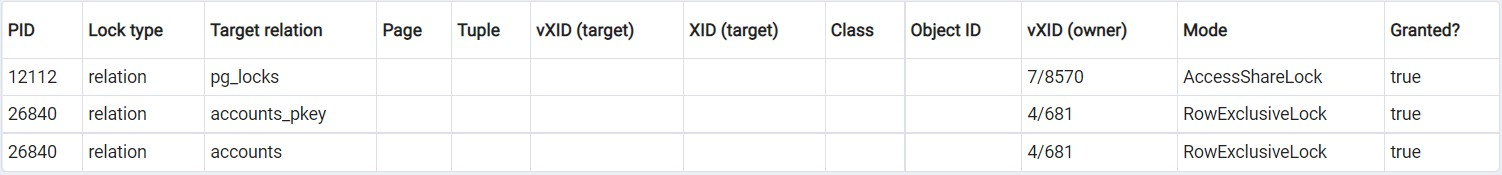
\includegraphics[width=1\textwidth]{figures/8-b-1.jpg}
    \caption
	{
لاگ پس از تغییر حساب \lr{Amir} و \lr{Ali} و پیش از پایان تراکنش(\lr{commit})
	}
    \label{fig:fig1}
\end{figure}
\begin{figure}[H]
    \centering
    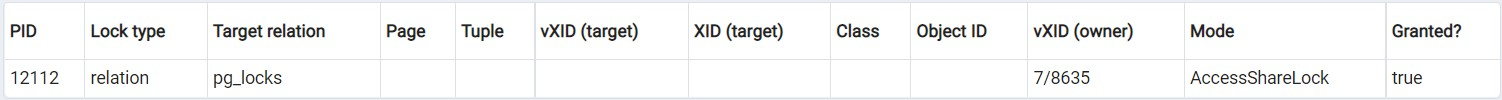
\includegraphics[width=1\textwidth]{figures/8-b-2.jpg}
    \caption
	{
لاگ پس از تغییر حساب \lr{Amir} و \lr{Ali} و پس از پایان تراکنش(\lr{commit})
	}
    \label{fig:fig1}
\end{figure}
\begin{figure}[H]
    \centering
    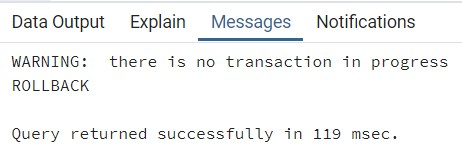
\includegraphics[width=1\textwidth]{figures/8-b-3.jpg}
    \caption
	{
پس از پایان تراکنش دیگر \lr{rollback} صورت نمی‌گیرد، زیرا تراکنش درحال اجرا نداریم.
	}
    \label{fig:fig1}
\end{figure}

\subsection{\lr{c}}
\begin{figure}[H]
    \centering
    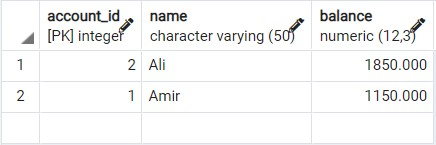
\includegraphics[width=1\textwidth]{figures/8-c-1.jpg}
    \caption
	{
جدول \lr{accounts} پس از تغییر حساب \lr{Amir} و \lr{Ali} و پیش از \lr{rollback}
	}
    \label{fig:fig1}
\end{figure}
\begin{figure}[H]
    \centering
    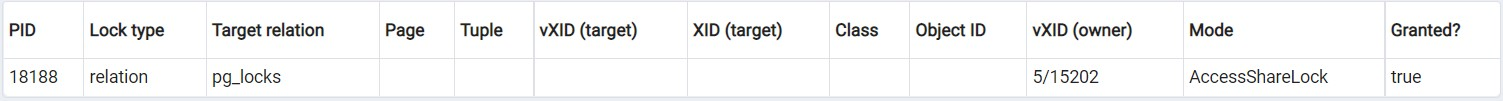
\includegraphics[width=1\textwidth]{figures/8-c-2.jpg}
    \caption
	{
لاگ پس از تغییر حساب \lr{Amir} و \lr{Ali} و پیش از \lr{rollback}
	}
    \label{fig:fig1}
\end{figure}
\begin{figure}[H]
    \centering
    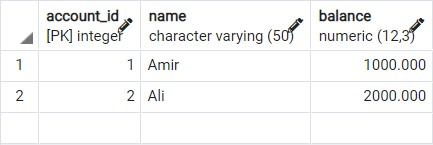
\includegraphics[width=1\textwidth]{figures/8-c-3.jpg}
    \caption
	{
جدول \lr{accounts} پس از تغییر حساب \lr{Amir} و \lr{Ali} و پس از \lr{rollback}
	}
    \label{fig:fig1}
\end{figure}
\begin{figure}[H]
    \centering
    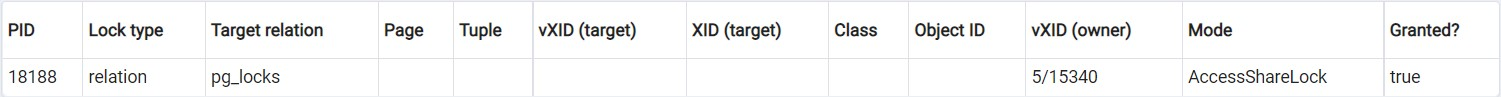
\includegraphics[width=1\textwidth]{figures/8-c-4.jpg}
    \caption
	{
لاگ پس از تغییر حساب \lr{Amir} و \lr{Ali} و پس از \lr{rollback}
	}
    \label{fig:fig1}
\end{figure}


\section{9}
\begin{figure}[H]
    \centering
    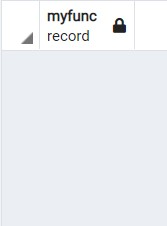
\includegraphics[width=0.7\textwidth]{figures/9-a.jpg}
    \caption
	{
خروجی اجرای تابع برای ناحیه \lr{Alberta}
	}
    \label{fig:fig1}
\end{figure}
\begin{figure}[H]
    \centering
    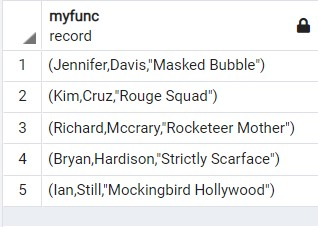
\includegraphics[width=0.7\textwidth]{figures/9-b.jpg}
    \caption
	{
خروجی اجرای تابع برای ناحیه \lr{Texas}
	}
    \label{fig:fig1}
\end{figure}


\section{10}
\begin{figure}[H]
    \centering
    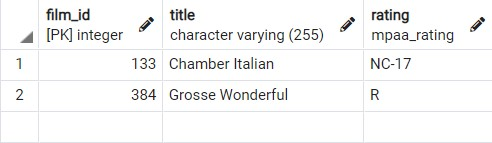
\includegraphics[width=0.7\textwidth]{figures/10-a.jpg}
    \caption
	{
قبل از اجرای \lr{stored procedure}
	}
    \label{fig:fig1}
\end{figure}
\begin{figure}[H]
    \centering
    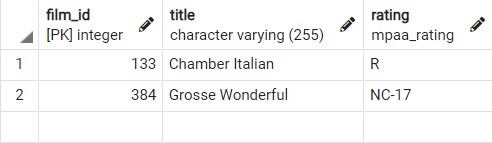
\includegraphics[width=0.7\textwidth]{figures/10-b.jpg}
    \caption
	{
پس از اجرای \lr{stored procedure}
	}
    \label{fig:fig1}
\end{figure}


%------------------------------------------------------------------------------------------


\section*{منابع}
\renewcommand{\section}[2]{}%
\begin{thebibliography}{99} % assumes less than 100 references
%چنانچه مرجع فارسی نیز داشته باشید باید دستور فوق را فعال کنید و مراجع فارسی خود را بعد از این دستور وارد کنید


\begin{LTRitems}

\resetlatinfont

\bibitem{b1} https://www.tutorialspoint.com/what-is-the-difference-between-blob-and-clob-datatypes
\end{LTRitems}

\end{thebibliography}


\end{document}
